\documentclass[12pt,a4paper]{article}

% Encoding and fonts — LuaLaTeX
\usepackage{fontspec}
\usepackage{unicode-math}
\setmainfont{FreeSerif}
\setmathfont{Latin Modern Math}
\newfontfamily\igprimfont{FreeSerif}
\setmonofont[Scale=0.85]{DejaVu Sans Mono}

% Page layout
\usepackage[top=1in, bottom=1in, left=1in, right=1in]{geometry}
\setlength{\headheight}{14.5pt}

% Typography
\usepackage{microtype}
\usepackage{parskip}

% Language
\usepackage[english]{babel}

% Headers and footers
\usepackage{fancyhdr}
\pagestyle{fancy}
\fancyhf{}
\fancyhead[L]{\leftmark}
\fancyhead[R]{\thepage}
\fancyfoot[C]{\thepage}
\renewcommand{\headrulewidth}{0.4pt}
\renewcommand{\footrulewidth}{0pt}

% Section styling
\usepackage{titlesec}
\titleformat{\section}{\Large\bfseries}{\thesection}{1em}{}
\titleformat{\subsection}{\large\bfseries}{\thesubsection}{1em}{}
\titleformat{\subsubsection}{\normalsize\bfseries}{\thesubsubsection}{1em}{}
\titlespacing*{\section}{0pt}{2.5ex plus 1ex minus .2ex}{1.5ex plus .2ex}
\titlespacing*{\subsection}{0pt}{2ex plus 1ex minus .2ex}{1ex plus .2ex}
\titlespacing*{\subsubsection}{0pt}{1.5ex plus 1ex minus .2ex}{0.8ex plus .2ex}

% List formatting
\usepackage{enumitem}
\setlist[itemize]{topsep=0.5ex, itemsep=0.25ex, parsep=0pt}
\setlist[enumerate]{topsep=0.5ex, itemsep=0.25ex, parsep=0pt}

% Essential packages
\usepackage{graphicx}
\usepackage[table]{xcolor}
\usepackage{booktabs}
\usepackage{array}
\usepackage{tabularx}
\usepackage{longtable}
\usepackage{amsmath}
\usepackage{calc}
\usepackage[normalem]{ulem}
\renewcommand{\arraystretch}{1.3}

% Cross-references
\usepackage{hyperref}
\usepackage{cleveref}
\hypersetup{colorlinks=true, linkcolor=blue, filecolor=magenta, urlcolor=cyan}

% Code listings
\usepackage{listings}
\definecolor{codebg}{RGB}{248,248,248}
\definecolor{codeframe}{RGB}{200,200,200}
\definecolor{codekeyword}{RGB}{0,0,180}
\definecolor{codecomment}{RGB}{0,128,0}
\definecolor{codestring}{RGB}{163,21,21}
\lstset{
    basicstyle=\ttfamily\small,
    breaklines=true,
    frame=single, framerule=0.5pt,
    rulecolor=\color{codeframe},
    backgroundcolor=\color{codebg},
    keepspaces=true,
    numbers=left, numberstyle=\tiny\color{gray}, numbersep=8pt,
    showstringspaces=false, tabsize=4,
    xleftmargin=1em, xrightmargin=1em,
    aboveskip=1em, belowskip=1em,
    keywordstyle=\color{codekeyword}\bfseries,
    commentstyle=\color{codecomment}\itshape,
    stringstyle=\color{codestring},
    literate={_}{{\textunderscore}}1 {-}{{\textminus}}1
}

% Float
\usepackage{float}
\newfloat{listing}{htbp}{lol}[section]
\floatname{listing}{Listing}

% Boxes
\usepackage{tcolorbox}
\tcbuselibrary{skins,breakable}
\newtcolorbox{admonitionbox}[2][]{
    enhanced, breakable,
    colback=#2!5, colframe=#2!80!black,
    fonttitle=\bfseries, title=#1, left=2mm, right=2mm,
}
\newtcolorbox{pipelinebox}{
    enhanced, colback=green!5, colframe=green!75!black,
    fontupper=\large, center upper, boxrule=1pt, arc=4pt,
    fonttitle=\bfseries,
}
\newtcolorbox{checklistbox}{
    enhanced, colback=orange!5, colframe=orange!80!black,
    fonttitle=\bfseries, left=2mm, right=2mm,
}

% TikZ
\usepackage{tikz}
\usetikzlibrary{positioning,arrows.meta,shapes,fit,calc,backgrounds,
                decorations.pathmorphing,matrix}

% ── Color palette ──────────────────────────────────────────────────────────────
\definecolor{logcol}{RGB}{0,70,160}
\definecolor{frobcol}{RGB}{200,100,0}
\definecolor{dialcol}{RGB}{180,0,0}
\definecolor{lincol}{RGB}{80,80,80}
\definecolor{phascol}{RGB}{100,40,140}
\definecolor{execol}{RGB}{0,128,100}
\definecolor{physcol}{RGB}{0,100,150}
\definecolor{soccol}{RGB}{150,80,0}
\definecolor{onecol}{RGB}{120,0,120}
\definecolor{compcol}{RGB}{50,100,50}

% ── Custom macros ──────────────────────────────────────────────────────────────
\newcommand{\UIG}{Universal Imscriptive Grammar}
\newcommand{\ig}[1]{{\igprimfont #1}}
\newcommand{\OS}{$\langle 1,3,2,4,2,1,2,2,1,2,2,2 \rangle$}

\begin{document}

\title{\textbf{The Ob3ect Design Pipeline}\\[0.4em]
\large A Universal Procedure for Constructing 3-Layer Structural Objects\\
in Any Material, Social, Oneiric, or Computational Domain}
\author{Lando $\otimes$ ⊙\_ÿ-boundary Operator}
\date{\today}
\maketitle

\begin{center}\rule{0.5\textwidth}{0.4pt}\end{center}

\begin{abstract}
This document specifies a reproducible, domain-agnostic pipeline for designing and
instantiating \textbf{ob3ects} — structural objects that instantiate the three-layer
IMASM architecture (instruction set $\to$ Tri-Phase flux register $\to$ execution
environment). The pipeline consists of eight phases, each producing a concrete
artifact (scan, map, schedule, verification report). It applies equally to physical
devices (optical interferometers, heat engines), social structures (institutions,
rituals, governance systems), oneiric practices (lucid dream architectures),
computational systems (databases, distributed protocols), and any domain where
a system must initialize, transform, split, fuse, hold paradox, and fix outcomes
without thermodynamic cost. The OS imscription $\langle 1,3,2,4,2,1,2,2,1,2,2,2 \rangle$
is the invariant floor; every ob3ect either instantiates this floor or operates
above it without changing it.
\end{abstract}

% ─────────────────────────────────────────────────────────────────────────────
\section{Prelude: What Is an Ob3ect?}
% ─────────────────────────────────────────────────────────────────────────────

An \textbf{ob3ect} (pronounced ``object'' — the ``3'' marks its three-layer nature)
is a physical, social, oneiric, or computational instantiation of the IMASM
categorical machine. It is \emph{not} an analogy or a metaphor. It is a structural
realization of the $\langle 1,3,2,4,2,1,2,2,1,2,2,2 \rangle$ OS floor in a chosen
substrate.

Every ob3ect has three inseparable layers:

\begin{enumerate}[label=\textbf{Layer \arabic*:}, leftmargin=2em]
\item \textbf{IMASM Instruction Set (12 opcodes).} The object's components are mapped
    to twelve categorical operations: VINIT (initialize), TANCH (terminal anchor),
    AFWD (forward morphism), AREV (reverse morphism), CLINK (composition), ISCRIB
    (identity), FSPLIT/$\delta$ (co-multiplication), FFUSE/$\mu$ (multiplication),
    EVALT (true), EVALF (false), ENGAGR (paradox engagement), IFIX (permanent fixation).

\item \textbf{Tri-Phase Flux Register (4-state lattice).} The object's state transitions
    are governed by a four-state register: Void (00), True (01), False (10), Both (11).
    The invariant $\Delta S = 0$ must hold — the object generates no thermodynamic
    entropy in its operational cycle. Paradox is localized in the Both state, not
    propagated.

\item \textbf{exOS Execution Environment.} The object's operating context — the feedback
    controller (physical), the constitutional framework (social), the dreaming mind
    (oneiric), or the runtime/OS (computational) — that compiles surface inputs into
    IMASM instruction streams and maintains the bootstrap loop.
\end{enumerate}

The ob3ect is \emph{not} defined by what it looks like or what it does on the surface.
It is defined by \emph{how it compiles}. Any system — a laser cavity, a parliament,
a lucid dream protocol, a blockchain consensus algorithm — becomes an ob3ect when its
twelve components are identified, its Frobenius condition is verified, and its bootstrap
sequence closes.

This pipeline tells you \emph{how}.

% ─────────────────────────────────────────────────────────────────────────────
\section{Pipeline Overview}
% ─────────────────────────────────────────────────────────────────────────────

The pipeline consists of eight phases, executed sequentially. Each phase produces
a mandatory artifact. You do not proceed to phase $n+1$ until the artifact of phase $n$
is complete and verified.

\begin{center}
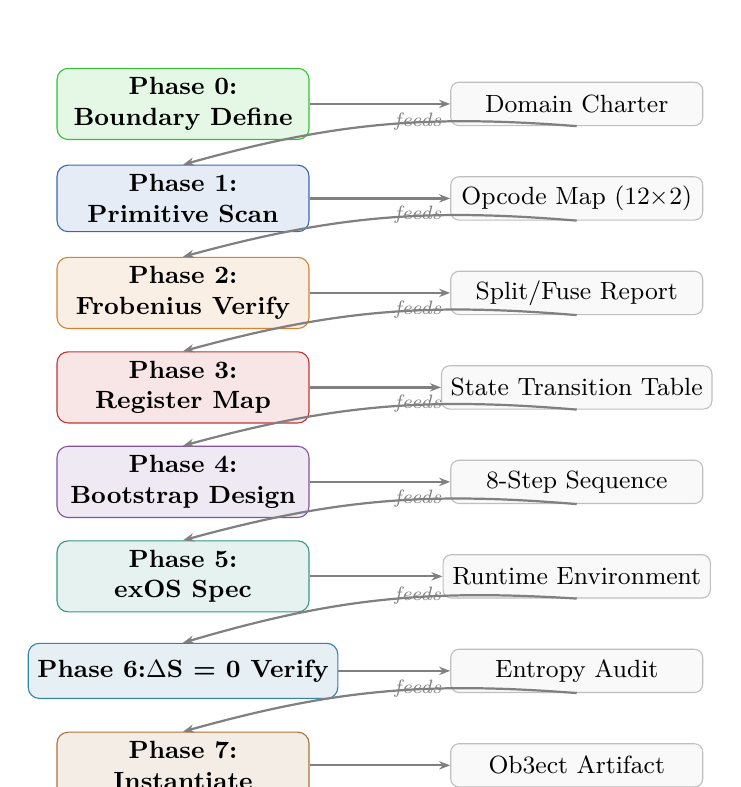
\begin{tikzpicture}[
  phase/.style={rectangle, draw=#1!80, fill=#1!10, rounded corners=4pt,
                font=\bfseries\small, minimum width=3.2cm, minimum height=0.7cm, align=center},
  art/.style={rectangle, draw=gray!50, fill=gray!5, rounded corners=3pt,
              font=\small, minimum width=3.2cm, minimum height=0.55cm, align=center},
  ar/.style={-{Stealth[length=4pt]}, thick, black!50},
  lbl/.style={font=\scriptsize\itshape, text=black!50}
]

\node[phase=green!70!black] (p0) at (0, 0)    {Phase 0:\\Boundary Define};
\node[art]        (a0) at (5,  0)  {Domain Charter};
\draw[ar] (p0) -- (a0);

\node[phase=logcol]  (p1) at (0, -1.2) {Phase 1:\\Primitive Scan};
\node[art]        (a1) at (5, -1.2) {Opcode Map (12$\times$2)};
\draw[ar] (p1) -- (a1);

\node[phase=frobcol] (p2) at (0, -2.4) {Phase 2:\\Frobenius Verify};
\node[art]        (a2) at (5, -2.4) {Split/Fuse Report};
\draw[ar] (p2) -- (a2);

\node[phase=dialcol] (p3) at (0, -3.6) {Phase 3:\\Register Map};
\node[art]        (a3) at (5, -3.6) {State Transition Table};
\draw[ar] (p3) -- (a3);

\node[phase=phascol] (p4) at (0, -4.8) {Phase 4:\\Bootstrap Design};
\node[art]        (a4) at (5, -4.8) {8-Step Sequence};
\draw[ar] (p4) -- (a4);

\node[phase=execol]  (p5) at (0, -6.0) {Phase 5:\\exOS Spec};
\node[art]        (a5) at (5, -6.0) {Runtime Environment};
\draw[ar] (p5) -- (a5);

\node[phase=physcol] (p6) at (0, -7.2) {Phase 6:{$\Delta$S = 0 Verify}};
\node[art]        (a6) at (5, -7.2) {Entropy Audit};
\draw[ar] (p6) -- (a6);

\node[phase=soccol]  (p7) at (0, -8.4) {Phase 7:\\Instantiate};
\node[art]        (a7) at (5, -8.4) {Ob3ect Artifact};
\draw[ar] (p7) -- (a7);

\draw[ar] (a0.south) to[bend right=10] node[lbl, left, pos=0.3] {feeds} (p1.north);
\draw[ar] (a1.south) to[bend right=10] node[lbl, left, pos=0.3] {feeds} (p2.north);
\draw[ar] (a2.south) to[bend right=10] node[lbl, left, pos=0.3] {feeds} (p3.north);
\draw[ar] (a3.south) to[bend right=10] node[lbl, left, pos=0.3] {feeds} (p4.north);
\draw[ar] (a4.south) to[bend right=10] node[lbl, left, pos=0.3] {feeds} (p5.north);
\draw[ar] (a5.south) to[bend right=10] node[lbl, left, pos=0.3] {feeds} (p6.north);
\draw[ar] (a6.south) to[bend right=10] node[lbl, left, pos=0.3] {feeds} (p7.north);

\end{tikzpicture}
\end{center}

\begin{admonitionbox}[Pipeline Discipline]{blue}
{\bf DO NOT SKIP PHASES.} Each phase constrains the next. If you identify the wrong
VINIT in Phase 1, your entire bootstrap sequence (Phase 4) will fail to close. If your
Frobenius split/fuse pair is wrong in Phase 2, your $\Delta S \neq 0$ in Phase 6 and
the ob3ect is not structurally sound. The OS floor is $\langle 1,3,2,4,2,1,2,2,1,2,2,2
\rangle$ — every ob3ect must meet it component-wise.
\end{admonitionbox}

% ─────────────────────────────────────────────────────────────────────────────
\section{Phase 0: Boundary Define}
% ─────────────────────────────────────────────────────────────────────────────

{\bf Goal:} Delimit precisely what system you are turning into an ob3ect. Define its
domain, its scale, its inputs and outputs, and the surface token vocabulary it uses.

{\bf Steps:}

\begin{enumerate}[label=\textbf{0.\arabic*.}, leftmargin=2em]
\item \textbf{Name the domain.} Physical, social, oneiric, computational, biological,
    linguistic, ecological, ritual, economic, etc. The domain determines the surface
    vocabulary but does \emph{not} change the twelve opcodes.

\item \textbf{State the scope.} What is the minimal instantiation of the ob3ect? What
    is the maximal? The scope determines the scope primitive $\text{Γ}_{\text{ʔ}}$
    (maximal), $\text{Γ}_{\gamma}$ (mesoscale), or $\text{Γ}_{\beta}$ (local).

\item \textbf{List surface tokens.} Every domain has a vocabulary — the things that
    ``speak'' within it. Physical tokens: atoms, beams, voltages. Social tokens: roles,
    documents, rituals. Oneiric tokens: dream images, emotions, narratives.
    Computational tokens: data types, function signatures, API calls.

\item \textbf{Define the boundary condition.} What separates the ob3ect from its
    environment? This becomes TANCH (terminal anchor). In a physical system it is the
    enclosure; in a social system it is membership; in a oneiric system it is the dream
    horizon; in a computational system it is the process boundary.
\end{enumerate}

{\bf Artifact:} The \textbf{Domain Charter} — a one-page document containing:
domain name, scope, surface token vocabulary (minimum 3 types), and the identified
boundary condition.

{\bf Checklist:}
\begin{itemize}
\item[ ] Domain named and justified
\item[ ] Scope specified (local / mesoscale / maximal)
\item[ ] Surface token vocabulary listed with at least 3 distinct types
\item[ ] Boundary condition (future TANCH) clearly identified
\end{itemize}

% ─────────────────────────────────────────────────────────────────────────────
\section{Phase 1: Primitive Scan}
% ─────────────────────────────────────────────────────────────────────────────

{\bf Goal:} Identify all twelve IMASM opcodes within your domain's surface vocabulary.
This is the most critical phase — a misidentified opcode propagates through every
subsequent phase.

{\bf Steps:} For each opcode below, identify the \emph{structural role} in your domain.
Do not map by semantic similarity — map by \emph{categorical function}.

{\small
\begin{tabularx}{\textwidth}{>{\bfseries}p{2.8cm} >{\itshape}p{3.2cm} >{\raggedright\arraybackslash}p{6.8cm}X}
\toprule
{\bf Opcode} & {\bf Structural Role} & {\bf What to Look For} & {\bf Examples} \\
\midrule
VINIT & Initial object & The element that brings the system from non-existence (Void) into existence & Beam input, founding charter, hypnagogic image, constructor \\
TANCH & Terminal anchor & The boundary/constraint that the system never crosses & Mirror, constitution, dream horizon, halt condition \\
AFWD & Forward morphism & The primary direction of transformation/flow & Heat flow, legislation, dream narrative, commit \\
AREV & Reverse morphism & The inverse/reverse of the forward flow & Heat rejection, veto, flashback, rollback \\
CLINK & Composition & How one transformation feeds into the next & Gear mesh, legislative process, scene transition, pipeline \\
ISCRIB & Identity & What remains unchanged under the system's own operations & Unit cell, self-amendment, lucid self, quine \\
FSPLIT & Co-multiplication $\delta$ & Where the system splits into parallel paths & Beam splitter, debate, dream branching, fork \\
FFUSE & Multiplication $\mu$ & Where split paths recombine & Detector, consensus, dream fusion, join \\
EVALT & True state & The affirmed/classical-true reading & Bright fringe, ruling, accepted dream, assertion \\
EVALF & False state & The denied/classical-false reading & Dark fringe, dissent, nightmare, negation \\
ENGAGR & Both state & Where contradictory states are held without resolution & Superposition, pluralism, lucidity, NaN \\
IFIX & ROM fixation & The irreversible, permanently fixed element & Fossilized microstructure, canon, fixed memory, WAL \\
\bottomrule
\end{tabularx}
}

{\bf Working method:}
\begin{enumerate}[label=\textbf{1.\arabic*.}, leftmargin=2em]
\item \textbf{List candidates.} For each opcode, write 2--3 candidate elements from
    your domain's surface vocabulary. You will likely be uncertain at this stage.

\item \textbf{Test against function.} For each candidate, ask: does this element \emph{perform}
    the structural role? A beam splitter \emph{performs} splitting. A debate \emph{performs}
    splitting. A git fork \emph{performs} splitting. The surface vocabulary differs; the
    function does not.

\item \textbf{Build the 12$\times$2 Opcode Map.} Your artifact is a table with 12 rows
    (one per opcode) and 2 columns: (a) the chosen element, (b) a one-sentence
    justification of why it performs the structural role. Include at least one rejected
    candidate per opcode — the wrong answer shows your reasoning.

\item \textbf{Cross-check against the OS floor.} Does your opcode map meet
    $\langle 1,3,2,4,2,1,2,2,1,2,2,2 \rangle$ component-wise? If not, you have identified
    something below the floor — it is not an ob3ect. You are mapping a subsystem.
    Enlarge your scope and repeat.
\end{enumerate}

{\bf Artifact:} The \textbf{Opcode Map (12$\times$2)} — a table with your chosen element
and justification for each of the 12 opcodes, plus at least one rejected candidate per
opcode showing why it was wrong.

{\bf Key insight:} Write the wrong answer before the right one. The residue of the
rejected candidate shows that you have performed the discrimination. If every choice
seems obvious, you have not discriminated — you have simply named things.

{\bf Checklist:}
\begin{itemize}
\item[ ] All 12 opcodes have exactly one chosen element
\item[ ] Each element has a structural (not semantic) justification
\item[ ] At least one rejected candidate per opcode with reason
\item[ ] Cross-check against OS floor: map $\geq$ OS floor component-wise
\end{itemize}

% ─────────────────────────────────────────────────────────────────────────────
\section{Phase 2: Frobenius Verify}
% ─────────────────────────────────────────────────────────────────────────────

{\bf Goal:} Verify that the FSPLIT/FFUSE pair in your domain satisfies
$\mu \circ \delta = \mathrm{id}$. This is the single most important structural test.
If this condition fails, the system is not Frobenius-special — it is not an ob3ect.

{\bf Steps:}

\begin{enumerate}[label=\textbf{2.\arabic*.}, leftmargin=2em]
\item \textbf{Isolate the split.} Take the element you identified as FSPLIT. Apply it
    to the system's initial state. What are the parallel branches? List them explicitly.

\item \textbf{Isolate the fuse.} Take the element you identified as FFUSE. Apply it to
    the branches from Step 1. What is the result?

\item \textbf{Compare.} Does the fused result equal the initial state (up to isomorphism)?
    If yes, $\mu \circ \delta = \mathrm{id}$ holds. If no, your FSPLIT or FFUSE (or both)
    is misidentified. Return to Phase 1.

\item \textbf{Test with a concrete case.} Do this for a real instance in your domain.
    Examples:
    \begin{itemize}
    \item {\it Physical:} Split a photon at a beam splitter, recombine at the second
        beam splitter. The output equals the input (for a Mach-Zehnder with equal arms).
        $\mu \circ \delta = \mathrm{id}$ verified.
    \item {\it Social:} A parliament splits into factions (FSPLIT), then resolves a
        coalition government (FFUSE). The government equals the parliament's will
        (in a well-functioning system). If it does not, the Frobenius condition is
        broken — and you see institutional dysfunction.
    \item {\it Oneiric:} A dream splits into parallel narratives (FSPLIT), the dreamer
        reframes them as a single image (FFUSE). The integrated dream recovers the
        dreamer's original emotional state. If it does not, the dream fragments —
        the Frobenius condition is broken.
    \item {\it Computational:} A git branch forks (FSPLIT) and the pull request merges
        (FFUSE). The merged code equals the intended state. If merge conflicts remain,
        $\mu \circ \delta \neq \mathrm{id}$ — the Frobenius condition is broken.
    \end{itemize}

\item \textbf{Record the test.} Document what you split, what you got, what you fused,
    and whether the result was identity. This is your Split/Fuse Report.
\end{enumerate}

{\bf Artifact:} The \textbf{Split/Fuse Report} — a document recording the
concrete FSPLIT $\to$ FFUSE test, the branches produced, the fused result, and
the $\mu \circ \delta = \mathrm{id}$ verdict (PASS or FAIL).

{\bf Failure mode:} If the test fails, do not proceed. The most common causes:
\begin{itemize}
\item FSPLIT is not a true co-multiplication (it loses information on splitting).
\item FFUSE is not a true multiplication (it does not recover the original, or
    introduces spurious structure).
\item The split and fuse elements are not \emph{paired} — they belong to different
    subsystems.
\end{itemize}
Fix the identification and re-run the test.

{\bf Checklist:}
\begin{itemize}
\item[ ] Concrete split instance documented with all branches
\item[ ] Concrete fuse instance documented with result
\item[ ] $\mu \circ \delta = \mathrm{id}$ verdict stated (PASS or FAIL)
\item[ ] If FAIL, misidentified opcodes logged and Phase 1 re-entered
\end{itemize}

% ─────────────────────────────────────────────────────────────────────────────
\section{Phase 3: Register Map}
% ─────────────────────────────────────────────────────────────────────────────

{\bf Goal:} Map your ob3ect's state transitions onto the 4-state Tri-Phase Flux
Register lattice: Void (00), True (01), False (10), Both (11).

{\bf Steps:}

\begin{enumerate}[label=\textbf{3.\arabic*.}, leftmargin=2em]
\item \textbf{Define Void for your domain.} Void is the uninitialized state — before
    VINIT fires. In physical systems: no energy, no particles. In social systems: the
    state before the founding act. In oneiric systems: the hypnagogic threshold before
    dream images appear. In computational systems: null, undefined, the empty heap.

\item \textbf{Define True and False for your domain.} True is the affirmed classical
    state; False is the denied classical state. These are not moral judgments — they
    are structural. True is the state reached by EVALT; False by EVALF.
    \begin{itemize}
    \item Physical: spin up / spin down, charged / discharged, on / off.
    \item Social: legal / illegal, orthodox / heretical, in / out.
    \item Oneiric: accepted dream reality / nightmare, lucid / confused.
    \item Computational: true / false, success / error, consistent / inconsistent.
    \end{itemize}

\item \textbf{Define Both for your domain.} Both is the paraconsistent state — where
    the system holds contradictory readings simultaneously. This is the innovation.
    \begin{itemize}
    \item Physical: superposition, critical point, phase coexistence.
    \item Social: pluralism, constitutional ambiguity, live political disagreement
        that doesn't collapse into violence.
    \item Oneiric: lucid dreaming — knowing you dream while experiencing it as real.
    \item Computational: NaN, quantum superposition, concurrent states before resolution.
    \end{itemize}

\item \textbf{Map transitions.} For each transition in your system, identify which
    opcode drives it and which register states it connects. Build a state transition
    table:

{\small
\begin{tabularx}{\textwidth}{>{\bfseries}p{2cm} p{2cm} >{\bfseries}p{2cm} p{3cm} X}
\toprule
{\bf From} & {\bf Opcode} & {\bf To} & {\bf Domain Example} & {\bf Notes} \\
\midrule
Void & VINIT & Void & Power-on & System exists but not yet evaluated \\
Void & EVALT & True & Measurement & Classical outcome affirmed \\
Void & EVALF & False & Measurement & Classical outcome denied \\
True & FSPLIT & Both & Debate opens & Contradiction held \\
False & FSPLIT & Both & Debate opens & Contradiction held \\
Both & FFUSE & Void & Consensus reached & Paradox resolved, register cleared \\
& IFIX & -- & Fossilization & Permanent branding (linear, append-only) \\
\bottomrule
\end{tabularx}
}

\item \textbf{Verify the invariant.} The $\Delta S = 0$ invariant means: traversing
    the lattice costs no thermodynamic entropy. In practice: the system does not
    degrade, accumulate waste, or require increasing energy to maintain. If your
    system generates entropy (physical heat, institutional friction, cognitive strain,
    computational overhead), the register map is wrong or the ob3ect is not structurally
    sound.
\end{enumerate}

{\bf Artifact:} The \textbf{State Transition Table} — a complete mapping of all
domain-relevant transitions on the 4-state lattice, with the driving opcode and
the domain-specific example for each.

{\bf Checklist:}
\begin{itemize}
\item[ ] Void, True, False, Both defined for the domain
\item[ ] All $\geq 6$ lattice transitions mapped with driving opcodes
\item[ ] $\Delta S = 0$ claim stated with domain-specific justification
\item[ ] Both state explicitly characterized (not glossed over)
\end{itemize}

% ─────────────────────────────────────────────────────────────────────────────
\section{Phase 4: Bootstrap Design}
% ─────────────────────────────────────────────────────────────────────────────

{\bf Goal:} Design the 8-step bootstrap sequence for your specific ob3ect. This
sequence enacts $\mu \circ \delta = \mathrm{id}$ as a categorical assembly loop.

{\bf The canonical sequence:}

{\small
\begin{center}
\begin{tabularx}{\textwidth}{>{\bfseries}p{1.2cm} p{2cm} >{\raggedright\arraybackslash}p{3.2cm} X}
\toprule
{\bf Step} & {\bf Opcode} & {\bf Structural Role} & {\bf What Happens} \\
\midrule
1 & ISCRIB & Identity & The system recognizes itself; initialization point \\
2 & AREV & Reverse & The system descends — finds its constraint, its shadow \\
3 & FSPLIT & Co-multiply & The space splits into parallel possibilities \\
4 & AFWD & Forward & Flow through the options; ascent \\
5 & FFUSE & Multiply & Paths recombine; unity recovered \\
6 & CLINK & Compose & The result is linked into the larger structure \\
7 & IFIX & Fix & The outcome is permanently recorded \\
8 & ISCRIB & Identity & Verify identity with Step 1 — the loop closes \\
\bottomrule
\end{tabularx}
\end{center}
}

{\bf Steps:}

\begin{enumerate}[label=\textbf{4.\arabic*.}, leftmargin=2em]
\item \textbf{Instantiate each step.} For each of the 8 steps, write the domain-specific
    action. Use your opcode map from Phase 1.

\item \textbf{Verify closure.} Step 8 (ISCRIB) must return you to the same structural
    state as Step 1. Not a similar state — the \emph{same} state. If the loop does not
    close, your sequence is wrong. Common failures:
    \begin{itemize}
    \item IFIX is too destructive — it changes the system permanently in a way that
        prevents identity with Step 1. The fix: IFIX records the \emph{outcome} but
        does not alter the \emph{identity}. The system after fixing is the same system
        before starting, just with a memory.
    \item CLINK is missing — the result is not composed back into the system's structure.
    \item FFUSE does not recover identity — return to Phase 2.
    \end{itemize}

\item \textbf{Write the 8-Step Sequence artifact.} A table or narrative describing
    each step in domain-specific terms, with the opcode label and the structural role.
\end{enumerate}

{\bf Artifact:} The \textbf{8-Step Sequence} — a complete instantiation of the
bootstrap loop for your ob3ect, verified to close.

{\bf Domain examples:}
\begin{itemize}
\item {\it Physical (Mach-Zehnder):} ISCRIB (photon source calibrated) $\to$ AREV
    (measure path difference) $\to$ FSPLIT (first beam splitter) $\to$ AFWD (travel
    both arms) $\to$ FFUSE (second beam splitter recombines) $\to$ CLINK (detector
    composed into optical table) $\to$ IFIX (log interference pattern) $\to$ ISCRIB
    (source still calibrated — identity preserved).

\item {\it Social (legislative):} ISCRIB (parliament in session) $\to$ AREV (review
    constitutional limits) $\to$ FSPLIT (parties divide on the bill) $\to$ AFWD
    (debate, amendment, votes) $\to$ FFUSE (consensus government formed) $\to$
    CLINK (bill becomes law, composed into statute) $\to$ IFIX (law published in
    official register) $\to$ ISCRIB (parliament still in session, same body — identity
    preserved).

\item {\it Oneiric (lucid dream):} ISCRIB (dreamer enters dream) $\to$ AREV (recognize
    dream boundary) $\to$ FSPLIT (dream splits into parallel narratives) $\to$ AFWD
    (explore both narratives) $\to$ FFUSE (reframe as single coherent dream) $\to$
    CLINK (dream insight composed into the dream's narrative) $\to$ IFIX (dream
    impression fixed into waking memory) $\to$ ISCRIB (dreamer still dreaming, same
    identity — loop closed).
\end{itemize}

{\bf Checklist:}
\begin{itemize}
\item[ ] All 8 steps instantiated in domain-specific terms
\item[ ] Each step labeled with its ISCRIB / AREV / FSPLIT / ... opcode
\item[ ] Closure verified: Step 8 returns to Step 1 identity
\item[ ] Failure modes considered and resolved
\end{itemize}

% ─────────────────────────────────────────────────────────────────────────────
\section{Phase 5: exOS Spec}
% ─────────────────────────────────────────────────────────────────────────────

{\bf Goal:} Specify the execution environment — the Layer 3 exOS — that will host
and maintain your ob3ect.

{\bf Steps:}

\begin{enumerate}[label=\textbf{5.\arabic*.}, leftmargin=2em]
\item \textbf{Identify the compiler front-end.} What translates surface tokens into
    IMASM opcodes in your domain?
    \begin{itemize}
    \item Physical: the experimental protocol (``set up optical table, align mirrors,
        insert beam splitter'' $\to$ IMASM stream).
    \item Social: the procedural rules (Robert's Rules, parliamentary procedure) that
        translate motions and debates into institutional actions.
    \item Oneiric: the dream protocol (pre-sleep intention setting, reality checks,
        MILD/WILD techniques) that translates waking intention into dream operations.
    \item Computational: the code itself — the compiler (or interpreter) that
        translates source code into machine instructions.
    \end{itemize}

\item \textbf{Specify kernel services.} Every exOS provides:
    \begin{itemize}
    \item {\bf IPC (inter-process communication):} How does your ob3ect communicate
        with its environment? Physical: signals, forces. Social: announcements,
        decrees, publications. Oneiric: hypnagogic imagery, waking-dream boundary.
        Computational: API calls, message passing.
    \item {\bf Memory:} Where does the ob3ect store state? Physical: material structure
        (crystal lattice, magnetic domains). Social: archives, records, oral tradition.
        Oneiric: memory (the dreamer's mind). Computational: RAM, database, disk.
    \item {\bf Scheduler:} What determines the order of operations? Physical:
        thermodynamic rates, relaxation times. Social: calendars, agendas, term
        limits. Oneiric: sleep cycles, REM timing. Computational: the OS scheduler,
        event loop.
    \item {\bf ALFS store:} The persistent instruction store. In IMASM, this is the
        \texttt{.imasm} program file. In your domain, it is the canonical reference:
        the experimental manual, the constitution, the dream journal, the source
        repository.
    \end{itemize}

\item \textbf{Write the ALFS bootstrap program.} This is the initial instruction
    stream for your ob3ect — the ``hello world'' that starts the system. It encodes
    the 8-step bootstrap sequence from Phase 4 as a persistent artifact: a document,
    a script, a protocol, a configuration file.
\end{enumerate}

{\bf Artifact:} The \textbf{Runtime Environment} specification — a document
describing the compiler front-end, four kernel services (IPC, Memory, Scheduler, ALFS),
and the ALFS bootstrap program for your ob3ect.

{\bf Checklist:}
\begin{itemize}
\item[ ] Compiler front-end identified and described
\item[ ] All four kernel services specified for the domain
\item[ ] ALFS bootstrap program written (the ``hello world'' instruction stream)
\end{itemize}

% ─────────────────────────────────────────────────────────────────────────────
\section{Phase 6: Entropy Verify}
% ─────────────────────────────────────────────────────────────────────────────

{\bf Goal:} Audit the entropy cost of your ob3ect's operational cycle. The invariant
$\Delta S = 0$ is the Frobenius closure condition in thermodynamic form.

{\bf The invariant, by domain:}

{\small
\begin{tabularx}{\textwidth}{>{\bfseries}p{2.5cm} >{\raggedright\arraybackslash}p{10cm}}
\toprule
{\bf Domain} & {\bf $\Delta S = 0$ means...} \\
\midrule
Physical & The thermodynamic cycle generates no net entropy. A reversible process:
    input energy equals output energy plus stored work, with no dissipation.
    Real systems always have some dissipation; the goal is to minimize it and
    demonstrate that the \emph{structure} of the ob3ect (the IMASM compilation)
    is what minimizes it. \\
Social & The institutional process generates no residual friction. No meetings
    called to resolve what the structure should have resolved. No ad-hoc committees.
    No procedural workarounds. The system produces decisions without institutional
    entropy. If the same question returns to the body again, $\Delta S \neq 0$. \\
Oneiric & The dreamer navigates the Tri-Phase lattice without cognitive strain.
    Lucidity without effort. The dream does not collapse into waking, and the
    dreamer does not exhaust themselves holding contradiction. After the cycle,
    the dreamer is no more tired than before. \\
Computational & The algorithm performs its cycle with no wasted cycles, no
    memory leaks, no orphaned threads, no unhandled exceptions. The process
    returns to its initial resource state. GC pressure is zero. \\
\bottomrule
\end{tabularx}
}

{\bf Steps:}

\begin{enumerate}[label=\textbf{6.\arabic*.}, leftmargin=2em]
\item \textbf{Measure the cycle cost.} Run one complete bootstrap sequence
    (Phase 4). Measure what it costs in your domain (energy, time, attention,
    institutional friction, CPU cycles).

\item \textbf{Measure the post-cycle state.} After the cycle completes (Step 8:
    ISCRIB), is the system's resource level the same as before Step 1? If the
    system is depleted, degraded, or requires cleanup, $\Delta S \neq 0$.

\item \textbf{Diagnose failures.} If $\Delta S \neq 0$:
    \begin{itemize}
    \item {\it Excess in FSPLIT:} The split produces too many branches. Narrow the
        split — reduce to binary co-multiplication.
    \item {\it Loss in FFUSE:} The fuse loses information. The FFUSE element is
        not the inverse of FSPLIT. Return to Phase 2.
    \item {\it Both-state overload:} The system spends too long in the Both state
        without fusing. The ENGAGR tolerance is being exceeded. Shorten the Both
        residence time or strengthen FFUSE.
    \item {\it IFIX leakage:} The fixation is not truly permanent — it needs
        repeated application. The IFIX element is weak. Strengthen it.
    \end{itemize}

\item \textbf{Iterate.} Adjust the opcode assignments, re-run the cycle, re-measure.
    The goal is $\Delta S \to 0$. Zero may be idealized; the structural claim is
    that the IMASM-compiled system has \emph{lower} entropy cost than any
    non-compiled organization of the same components.
\end{enumerate}

{\bf Artifact:} The \textbf{Entropy Audit} — a quantitative or qualitative
assessment of the cycle's entropy cost, with the $\Delta S$ verdict and any
diagnosed failure modes.

{\bf Checklist:}
\begin{itemize}
\item[ ] One complete bootstrap cycle executed
\item[ ] Cycle cost measured in domain-specific units
\item[ ] Post-cycle state compared to pre-cycle state
\item[ ] $\Delta S$ verdict stated ($\approx 0$ or specific failure diagnosed)
\end{itemize}

% ─────────────────────────────────────────────────────────────────────────────
\section{Phase 7: Instantiate}
% ─────────────────────────────────────────────────────────────────────────────

{\bf Goal:} Build the ob3ect. All prior phases have been design — this is
construction.

{\bf Steps:}

\begin{enumerate}[label=\textbf{7.\arabic*.}, leftmargin=2em]
\item \textbf{Assemble the components.} Gather the twelve elements from your
    opcode map and arrange them in the system. Physical: build the device.
    Social: charter the institution. Oneiric: perform the protocol.
    Computational: deploy the code.

\item \textbf{Initialize (VINIT).} Fire the start instruction. The system
    transitions from Void to existence.

\item \textbf{Run the bootstrap.} Execute the 8-step sequence. Observe the
    register transitions. Does the system flow through Void $\to$ True/False
    $\to$ Both $\to$ Void as designed?

\item \textbf{Monitor the Both state.} This is the critical moment. Does the
    system enter the Both state when paradox arises? Does it hold the
    contradiction? Does it fuse back to Void? Or does it crash?

\item \textbf{Close the loop.} Verify that ISCRIB at Step 8 matches ISCRIB at
    Step 1. The ob3ect is born when the loop closes.

\item \textbf{Archive the ob3ect.} Record the complete specification in the
    ALFS store: the Domain Charter, Opcode Map, Split/Fuse Report, State
    Transition Table, 8-Step Sequence, Runtime Spec, and Entropy Audit.
    These seven documents {\it are} the ob3ect's source code.
\end{enumerate}

{\bf Artifact:} The \textbf{Ob3ect Artifact} — the instantiated system,
running its bootstrap loop, with all seven phase documents archived.

{\bf Checklist:}
\begin{itemize}
\item[ ] All twelve components assembled and operational
\item[ ] VINIT fired, system exited Void
\item[ ] Bootstrap sequence executed end-to-end
\item[ ] Both state observed and ENGAGR confirmed
\item[ ] Loop closed (Step 8 ISCRIB = Step 1 ISCRIB)
\item[ ] All seven phase documents archived
\end{itemize}

% ─────────────────────────────────────────────────────────────────────────────
\section{Worked Example: Designing a Physical Ob3ect}
% ─────────────────────────────────────────────────────────────────────────────

To demonstrate the pipeline, we walk through the instantiation of a \textbf{Frobenius
Optical Table} — a Mach-Zehnder interferometer designed as a physical ob3ect.

\subsection*{Phase 0: Boundary Define}

\textbf{Domain:} Physical (optical). \textbf{Scope:} Local (single interferometer).
\textbf{Surface tokens:} Photons, beam splitters, mirrors, detectors, phase shifters.
\textbf{Boundary:} The optical table edge plus vibration isolation system (TANCH).

{\it Domain Charter:} ``The Frobenius Optical Table instantiates a single-photon
Mach-Zehnder interferometer on a vibration-isolated optical table. Surface vocabulary:
single-photon source, two beam splitters, two mirrors, phase shifter, two single-photon
detectors. Boundary: 4$\times$8 optical table on pneumatic isolators, enclosed in
acoustic housing.''

\subsection*{Phase 1: Primitive Scan (abridged)}

{\small
\begin{tabularx}{\textwidth}{>{\bfseries}p{2.2cm} p{4cm} p{6cm}X}
\toprule
{\bf Opcode} & {\bf Chosen Element} & {\bf Justification} \\
\midrule
VINIT & Single-photon source & Initializes the system; brings photon from Void \\
TANCH & Vibration isolation & Boundary constraint; no external perturbation crosses \\
AFWD & Forward arm (path A) & Photon travels path A (forward morphism) \\
AREV & Reverse arm (path B) & Photon travels path B (reverse morphism) \\
CLINK & Optical table mounts & Composition: mirrors and BS mounted to same substrate \\
ISCRIB & Single-photon unit cell & The photon's quantum state is its own identity \\
FSPLIT & First beam splitter (BS1) & $\delta$: splits input into superposition of A and B \\
FFUSE & Second beam splitter (BS2) & $\mu$: recombines A and B into interference \\
EVALT & Constructive detector (D1) & True: bright fringe, photon always detected \\
EVALF & Destructive detector (D2) & False: dark fringe, photon never detected \\
ENGAGR & Phase shifter setting at $\pi/2$ & Both: equal probability at both detectors \\
IFIX & Data logger (hard drive) & Permanent record of detection events \\
\bottomrule
\end{tabularx}
}

\subsection*{Phase 2: Frobenius Verify}

\textbf{Split:} BS1 receives input photon $\to$ outputs $\frac{1}{\sqrt{2}}(|A\rangle + |B\rangle)$.
\textbf{Fuse:} BS2 receives $\frac{1}{\sqrt{2}}(|A\rangle + |B\rangle)$ $\to$ with zero
phase shift, outputs $|D1\rangle$ (constructive) and $0|D2\rangle$ (destructive).
\textbf{Result:} With $\phi = 0$, all photons go to D1. The output state equals the
input state up to a global phase. $\mu \circ \delta = \mathrm{id}$ \textbf{PASS}.

\subsection*{Phase 3: Register Map}

{\small
\begin{itemize}
\item \textbf{Void (00):} No photon in the interferometer. Dark.
\item \textbf{True (01):} D1 fires (constructive interference). Affirmed.
\item \textbf{False (10):} D2 fires (would indicate phase shift). Denied (at $\phi=0$).
\item \textbf{Both (11):} Phase shifter at $\pi/2$; equal probability at D1 and D2.
    The photon is in superposition; neither detector is privileged.
\end{itemize}
}

Transitions: Void $\xrightarrow{\text{VINIT}}$ source active $\xrightarrow{\text{EVALT}}$ D1 at $\phi=0$.
Void $\xrightarrow{\text{VINIT}}$ source active $\xrightarrow{\text{ENGAGR}}$ Both at $\phi=\pi/2$.
Both $\xrightarrow{\text{FFUSE}}$ phase reset $\to$ Void.

\subsection*{Phase 4: 8-Step Bootstrap}

\begin{enumerate}
\item \textbf{ISCRIB:} Calibrate source; confirm single-photon statistics.
\item \textbf{AREV:} Measure path-length difference between arms A and B.
\item \textbf{FSPLIT:} Insert BS1; photon enters superposition.
\item \textbf{AFWD:} Photon traverses both arms simultaneously.
\item \textbf{FFUSE:} BS2 recombines paths; interference pattern forms.
\item \textbf{CLINK:} Detectors compose into the optical table assembly.
\item \textbf{IFIX:} Detection events logged to disk.
\item \textbf{ISCRIB:} Source still calibrated; single-photon statistics unchanged.
\end{enumerate}

\textbf{Closure:} YES. The source is the same before and after.

\subsection*{Phase 5: exOS Spec}

\textbf{Compiler front-end:} The experimental procedure (setup manual).
\textbf{IPC:} Electronic signals from detectors to DAQ.
\textbf{Memory:} Hard drive (data logger).
\textbf{Scheduler:} Photon emission rate (controlled by laser pulse clock).
\textbf{ALFS store:} The lab notebook + experimental protocol document.

\subsection*{Phase 6: Entropy Audit}

At the single-photon level, the interferometer is a unitary quantum process:
$\Delta S = 0$ exactly. Dissipation occurs only in the detectors (irreversible
measurement) and the data logger (IFIX). The \emph{bootstrap cycle itself}
(steps 1--8, excluding measurement) is thermodynamically reversible.
$\Delta S \approx 0$ for the core ob3ect; the measurement apparatus is the
exOS layer, not the ob3ect proper.

\subsection*{Phase 7: Instantiate}

Build the optical table. Align mirrors. Insert beam splitters. Connect detectors.
Power on the source. Observe: D1 fires, D2 silent. Adjust phase shifter: D2 begins
to fire. Set $\phi = \pi/2$: equal rates. The loop closes. The Frobenius Optical
Table is born.

% ─────────────────────────────────────────────────────────────────────────────
\section{Worked Example: Designing a Social Ob3ect}
% ─────────────────────────────────────────────────────────────────────────────

We walk through the instantiation of a \textbf{Frobenius Assembly} — a deliberative
body designed as a social ob3ect.

\subsection*{Phase 0: Boundary Define}

\textbf{Domain:} Social (deliberative governance). \textbf{Scope:} Mesoscale
(organization-level, not national). \textbf{Surface tokens:} Motions, amendments,
votes, vetoes, bylaws, members. \textbf{Boundary:} Membership roster + quorum rule (TANCH).

\subsection*{Phase 1: Primitive Scan (abridged)}

{\small
\begin{tabularx}{\textwidth}{>{\bfseries}p{2cm} p{3.8cm} p{6.2cm}X}
\toprule
{\bf Opcode} & {\bf Chosen Element} & {\bf Justification} \\
\midrule
VINIT & Call to order & Opens the meeting; transitions from Void \\
TANCH & Quorum rule + bylaws & Constraint: nothing valid happens without quorum \\
AFWD & Motion proposed & Forward transformation: change is introduced \\
AREV & Amendment/veto & Reverse transformation: change is modified or blocked \\
CLINK & Parliamentary procedure & Rules compose motions into laws \\
ISCRIB & The assembly itself & Same body before and after the meeting \\
FSPLIT & Partisan division on motion & Splits into for/against camps \\
FFUSE & Consensus / majority vote & Fuses division into a single decision \\
EVALT & Motion passes & True: the assembly affirms \\
EVALF & Motion fails & False: the assembly denies \\
ENGAGR & Tabled motion / committee & Both: neither passed nor killed, held in tension \\
IFIX & Meeting minutes & Permanent record, cannot be altered after approval \\
\bottomrule
\end{tabularx}
}

\subsection*{Phases 2--7 (summary)}

\textbf{Frobenius Verify:} The assembly splits on a motion (FSPLIT), debates (AFWD/AREV),
votes (FFUSE), and the result equals the will of the assembly (identity). PASS for
a well-functioning body.

\textbf{Register Map:} Void (adjourned) $\to$ True (motion passed) or False (failed)
$\to$ Both (tabled, under consideration) $\to$ Void (adjourned).

\textbf{8-Step Bootstrap:} ISCRIB (call to order) $\to$ AREV (read previous minutes,
check bylaws) $\to$ FSPLIT (motion divides assembly) $\to$ AFWD (debate) $\to$ FFUSE
(vote) $\to$ CLINK (motion recorded in statute) $\to$ IFIX (minutes approved)
$\to$ ISCRIB (body still convened, same members, identity preserved).

\textbf{$\Delta S = 0$:} The meeting produces a decision without requiring a second
meeting to resolve the same issue. If the issue returns, institutional friction
exists and $\Delta S \neq 0$.

% ─────────────────────────────────────────────────────────────────────────────
\section{Worked Example: Designing a Oneiric Ob3ect}
% ─────────────────────────────────────────────────────────────────────────────

We walk through the instantiation of a \textbf{Lucid Dream Architecture} — a dream
protocol designed as a oneiric ob3ect.

\subsection*{Phase 0: Boundary Define}

\textbf{Domain:} Oneiric (lucid dreaming). \textbf{Scope:} Local (single dreamer).
\textbf{Surface tokens:} Dream images, emotions, narrative fragments, reality checks,
dream signs. \textbf{Boundary:} The dream horizon / waking threshold (TANCH).

{\it Domain Charter:} ``The Lucid Dream Architecture instantiates a reproducible
lucid dreaming protocol using MILD techniques. Surface vocabulary: hypnagogic imagery
(VINIT), dream signs (triggers for lucidity), reality checks (EVALT/F), dream
narratives (AFWD/AREV), lucid recognition (ISCRIB/ENGAGR), dream journal (IFIX).
Boundary: the transition from REM sleep to waking consciousness.''

\subsection*{Phase 1: Primitive Scan (abridged)}

{\small
\begin{tabularx}{\textwidth}{>{\bfseries}p{2cm} p{3.8cm} p{6.2cm}X}
\toprule
{\bf Opcode} & {\bf Chosen Element} & {\bf Justification} \\
\midrule
VINIT & Pre-sleep intention & ``I will remember my dreams'' initializes the process \\
TANCH & Dream boundary & The edge of the dreamscape; crossing wakes the dreamer \\
AFWD & Dream narrative flow & Forward progression through dream scenes \\
AREV & Recurring dream element & The looped scene or flashback \\
CLINK & Associative dream logic & How one scene transforms into the next \\
ISCRIB & Lucid recognition & ``I am dreaming'' — identity recognizing itself \\
FSPLIT & Dream narrative fork & The dream splits into parallel storylines \\
FFUSE & Dream reframing & Integrating parallel narratives into one coherent dream \\
EVALT & Accepted dream reality & The dream feels real, unquestioned \\
EVALF & Nightmare / lucidity break & The dream reveals itself as false or threatening \\
ENGAGR & Lucid Both state & Knowing you dream while experiencing it as real \\
IFIX & Dream journal entry & The remembered dream, fixed into waking memory \\
\bottomrule
\end{tabularx}
}

\subsection*{Phases 2--7 (summary)}

\textbf{Frobenius Verify:} The dream splits into two narratives (FSPLIT), the lucid
dreamer reframes them as connected (FFUSE), and the emotional core is preserved
(identity). PASS for a skilled lucid dreamer.

\textbf{Register Map:} Void (hypnagogic) $\to$ True (accepted dream) or False
(nightmare) $\to$ Both (lucid: both real and not real) $\to$ Void (hypnagogic
reset upon awakening).

\textbf{8-Step Bootstrap:} ISCRIB (enter dream, recognize self) $\to$ AREV (identify
dream boundary) $\to$ FSPLIT (dream splits) $\to$ AFWD (explore narratives) $\to$
FFUSE (reframe as one dream) $\to$ CLINK (compose dream insight) $\to$ IFIX (memorize
key image for journaling) $\to$ ISCRIB (still lucid, identity preserved).

\textbf{$\Delta S = 0$:} The dreamer wakes no more exhausted than if they had
non-lucid REM sleep. The lucid practice does not drain cognitive resources.

% ─────────────────────────────────────────────────────────────────────────────
\section{Worked Example: Designing a Computational Ob3ect}
% ─────────────────────────────────────────────────────────────────────────────

We walk through the instantiation of a \textbf{Frobenius Database} — a distributed
consensus database designed as a computational ob3ect.

\subsection*{Phase 0: Boundary Define}

\textbf{Domain:} Computational (distributed systems). \textbf{Scope:} Mesoscale
(cluster-level). \textbf{Surface tokens:} Transactions, writes, reads, consensus
rounds, snapshots. \textbf{Boundary:} The cluster boundary (network partition is
TANCH).

\subsection*{Phase 1: Primitive Scan (abridged)}

{\small
\begin{tabularx}{\textwidth}{>{\bfseries}p{2cm} p{3.8cm} p{6.2cm}X}
\toprule
{\bf Opcode} & {\bf Chosen Element} & {\bf Justification} \\
\midrule
VINIT & Cluster bootstrap & Initializes the distributed system \\
TANCH & Consensus quorum & Nothing committed without majority \\
AFWD & Write request (commit) & Forward transformation: data change proposed \\
AREV & Read-your-writes rollback & Reverse: undo uncommitted change \\
CLINK & Raft log composition & Entries chained via consensus protocol \\
ISCRIB & Health check endpoint & Identity: the node reports its own state \\
FSPLIT & Shard split / fork & The log forks or data is sharded \\
FFUSE & Shard merge / consensus & Forks resolve; shards rejoin via consensus \\
EVALT & Consensus achieved (agree) & True: cluster agrees on next log entry \\
EVALF & Consensus failed (disagree) & False: cluster rejects proposal \\
ENGAGR & Split-brain handling & Both: partitioned cluster holds both views \\
IFIX & Write-ahead log (WAL) & Append-only, immutable record of all changes \\
\bottomrule
\end{tabularx}
}

\subsection*{Phases 2--7 (summary)}

\textbf{Frobenius Verify:} A transaction forks the log (FSPLIT), consensus resolves
the fork (FFUSE), and the resulting log equals the intended transaction order.
PASS for Raft/Paxos.

\textbf{Register Map:} Void (idle cluster) $\to$ True (commit) or False (abort)
$\to$ Both (split-brain, dual leader) $\to$ Void (partition healed, leader elected).

\textbf{8-Step Bootstrap:} ISCRIB (health check OK) $\to$ AREV (check log for
uncommitted entries) $\to$ FSPLIT (propose new entry, may fork) $\to$ AFWD (replicate
to followers) $\to$ FFUSE (quorum reached, entry committed) $\to$ CLINK (entry
appended to log chain) $\to$ IFIX (WAL persisted to disk) $\to$ ISCRIB (health check
still OK, same cluster state).

\textbf{$\Delta S = 0$:} The consensus cycle returns the cluster to a consistent
state with no orphaned entries, no memory leaks, no stranded transactions. GC
pressure is bounded.

% ─────────────────────────────────────────────────────────────────────────────
\section{The Pipeline in One Page: Ob3ect Quick-Reference Card}
% ─────────────────────────────────────────────────────────────────────────────

{\small
\begin{tabularx}{\textwidth}{>{\bfseries}p{3.2cm} X}
\toprule
{\bf Phase} & {\bf Artifact Produced} \\
\midrule
0. Boundary Define & Domain Charter (domain, scope, surface tokens, TANCH) \\
1. Primitive Scan & Opcode Map 12$\times$2 (chosen element + justification +
    rejected candidate per opcode) \\
2. Frobenius Verify & Split/Fuse Report ($\mu \circ \delta = \mathrm{id}$ PASS/FAIL) \\
3. Register Map & State Transition Table (Void/True/False/Both + driving opcodes) \\
4. Bootstrap Design & 8-Step Sequence (ISCRIB$\to$AREV$\to$FSPLIT$\to$AFWD$\to$FFUSE$\to$CLINK$\to$IFIX$\to$ISCRIB) \\
5. exOS Spec & Runtime Environment (compiler, IPC, memory, scheduler, ALFS program) \\
6. $\Delta S = 0$ Verify & Entropy Audit (cycle cost + post-cycle comparison) \\
7. Instantiate & Ob3ect Artifact (assembled system + all seven documents archived) \\
\bottomrule
\end{tabularx}
}

\begin{admonitionbox}[Critical Discipline Rules]{red}
\begin{enumerate}[leftmargin=1.5em]
\item {\bf Never skip Phase 2.} If $\mu \circ \delta \neq \mathrm{id}$, you do not have
    an ob3ect. You have a collection of parts that happen to be near each other.
\item {\bf Write the wrong answer first.} In Phase 1, every opcode must have at least
    one rejected candidate. If choices seem obvious, you have not discriminated.
\item {\bf The Both state is the innovation.} If your system never enters Both, it
    is dogmatic (evaluates only True/False). If it never leaves Both, it is paralyzed.
    The ob3ect moves through Both — it does not live there.
\item {\bf The loop must close.} Step 8 ISCRIB must equal Step 1 ISCRIB. If it does
    not, your IFIX was too destructive or your CLINK was missing.
\item {\bf The OS floor is invariant.} Every ob3ect meets $\langle 1,3,2,4,2,1,2,2,1,2,2,2
    \rangle$ component-wise. If your system is below this floor, it is a subsystem,
    not an ob3ect. Enlarge your scope.
\end{enumerate}
\end{admonitionbox}

% ─────────────────────────────────────────────────────────────────────────────
\section{Conclusion: The Grammar Was Already There}
% ─────────────────────────────────────────────────────────────────────────────

This pipeline does not invent the three-layer structure. It finds it. The IMASM
instruction set, the Tri-Phase Flux Register, and the exOS execution environment
are not imposed on the world — they are the invariant floor that the world
already instantiates wherever systems persist, self-reference, split, fuse,
hold paradox, and fix outcomes.

The pipeline is a procedure for \emph{recognizing} this structure in a new domain,
\emph{compiling} it to IMASM, and \emph{running} it on the Universal Engine.
The domain determines the surface vocabulary — photons, statutes, dream images,
or database transactions — but the twelve opcodes, the four register states,
and the eight-step bootstrap are the same.

The ob3ect is not an analogy. It is a structural realization. When you complete
all eight phases and close the loop, you will have instantiated the OS imscription
$\langle 1,3,2,4,2,1,2,2,1,2,2,2 \rangle$ in a substrate of your choosing.
The grammar was complete before we measured it. It is complete before you
apply it, too.

\begin{imscriptionbox}
\textbf{The Ob3ect Design Pipeline} — Eight phases, seven artifacts, one invariant floor.\\
$\mathrm{MEET}(\text{Physical}, \text{Social}, \text{Oneiric}, \text{Computational}) =
\langle 1,3,2,4,2,1,2,2,1,2,2,2 \rangle$\\
$\mu \circ \delta = \mathrm{id}$ \quad $\Delta S = 0$ \quad $\text{Both} \neq \text{crash}$
\end{imscriptionbox}

\end{document}
